% !TEX TS-program = pdflatex
\documentclass[11pt]{article}

% -------------------- Packages --------------------
\usepackage[a4paper,margin=1in]{geometry}
\usepackage{amsmath,amssymb}
\usepackage[T1]{fontenc}
\usepackage{lmodern}
\usepackage[table]{xcolor}
\usepackage{tcolorbox}
\tcbuselibrary{skins,breakable}
\usepackage{enumitem}
\usepackage{hyperref}

% --- Tables & Diagrams ---
\usepackage{booktabs}
\usepackage{array}
\usepackage{colortbl}
\usepackage{tikz}
\usetikzlibrary{calc,arrows.meta}
\usepackage{pgfplots}
\pgfplotsset{compat=1.18}

\pagestyle{empty}

% -------------------- Dark Theme Colors --------------------
\definecolor{bg}{HTML}{000000}
\definecolor{pairbg}{HTML}{121212}
\definecolor{solbg}{HTML}{0A0A0A}
\definecolor{border}{HTML}{2A2A2A}
\definecolor{text}{HTML}{FFFFFF}
\definecolor{muted}{HTML}{C9CDD3}
\definecolor{gold}{HTML}{FFD700}
\definecolor{green}{HTML}{4ADE80}
\definecolor{cyan}{HTML}{38BDF8}
\definecolor{redacc}{HTML}{F87171}

\definecolor{tablehead}{HTML}{1B1B1B}
\definecolor{tablerow}{HTML}{101010}

\pagecolor{bg}
\color{text}

\hypersetup{
  colorlinks=true,
  linkcolor=cyan,
  urlcolor=cyan
}

\setlength{\parindent}{0pt}
\setlength{\parskip}{10pt}

\setlist[itemize]{left=1.4em,itemsep=6pt,topsep=6pt}
\setlist[enumerate]{left=1.6em,itemsep=4pt,topsep=4pt}
% -------------------- tcolorbox Base --------------------
\tcbset{
  enhanced,
  breakable,
  arc=12pt,
  boxrule=0.8pt,
  left=16pt,right=16pt,top=12pt,bottom=12pt
}

% -------------------- FIXED BOXES (title bar not orange) --------------------
\newtcolorbox{QAPair}[1]{%
  colback=pairbg,
  colbacklower=solbg,
  colframe=border,
  coltext=text,
  title={#1},
  coltitle=gold,
  colbacktitle=pairbg, % <--- FIX: dark title bar
  boxed title style={colback=pairbg, colframe=border},
  fonttitle=\bfseries,
  segmentation style={draw=border, dashed, line width=0.6pt},
}

\newtcolorbox{QuickBox}{%
  colback=pairbg,
  colframe=cyan,
  coltext=text,
  colbacktitle=pairbg, % safe even if you add a title later
  coltitle=cyan,
  boxed title style={colback=pairbg, colframe=cyan},
  fontupper=\color{text},
  borderline north={4pt}{0pt}{cyan},
  arc=14pt,
  boxrule=0.8pt
}

% Small box for each subpart
\newtcolorbox{PartBox}[1]{%
  colback=solbg,
  colframe=cyan,
  coltext=text,
  title={#1},
  coltitle=gold,
  colbacktitle=pairbg, % <--- FIX: dark title bar
  boxed title style={colback=pairbg, colframe=cyan},
  fonttitle=\bfseries,
  arc=10pt,
  boxrule=0.8pt,
  left=14pt,right=14pt,top=10pt,bottom=10pt
}

% Setup box (the one that looked orange)
\newtcolorbox{SetupBox}[1]{%
  colback=pairbg,
  colframe=gold,
  coltext=text,
  title={#1},
  coltitle=gold,
  colbacktitle=pairbg, % <--- FIX: dark title bar
  boxed title style={colback=pairbg, colframe=gold},
  fonttitle=\bfseries,
  arc=10pt,
  boxrule=0.8pt,
  left=14pt,right=14pt,top=10pt,bottom=10pt
}

% Helpers
\newcommand{\Step}[1]{\textcolor{muted}{\textbf{Step #1:}}}
\newcommand{\Pof}[1]{\mathrm{P}\!\left(#1\right)}
\newcommand{\Samp}{\mathcal{S}}

% -------------------- pgfplots dark styling --------------------
\pgfplotsset{
  every axis/.append style={
    axis line style={color=text},
    tick style={color=text},
    ticklabel style={color=text},
    label style={color=text},
    title style={color=text},
    grid style={color=border},
    legend style={draw=border, fill=pairbg, text=text},
  }
}

% Nice tables on dark background
\newcommand{\DarkTable}{%
  \rowcolors{2}{tablerow}{solbg}
  \renewcommand{\arraystretch}{1.2}
  \setlength{\tabcolsep}{10pt}
}

% Tiny tiles for quick visuals
\tikzset{
  tile/.style={draw=cyan, rounded corners=3pt, line width=0.6pt, fill=solbg, minimum width=10mm, minimum height=8mm, align=center, text=text}
}

% ============================================================
\begin{document}

\begin{center}
{\LARGE\bfseries \textcolor{gold}{Exercise 11.3 --- Probability (Solutions)}}\\[-2pt]
\end{center}

\begin{QuickBox}
{\color{cyan}\bfseries Quick idea (very easy)}\par\medskip
\begin{itemize}
\item \textbf{Probability} means: \textbf{how many ways we can win} divided by \textbf{total possible ways}.
\[
\Pof{E}=\frac{\text{favourable outcomes}}{\text{total outcomes}}
\]
\item \textbf{Complement:} “not $E$” means everything except $E$:
\[
\Pof{\text{not }E}=1-\Pof{E}
\]
\item \textbf{Expected frequency:} if we repeat $N$ times:
\[
\text{Expected} = N \times \Pof{E}
\]
\end{itemize}
\end{QuickBox}

% ============================================================
% Q1
\begin{QAPair}{Question 1}
\textcolor{gold}{\bfseries Question:} A letter is chosen randomly from the word \texttt{ALLAH}. Find the probability of getting:
(i) a vowel \quad (ii) an H \quad (iii) an L \quad (iv) a consonant
\tcblower
\textcolor{green}{\bfseries Answer:}

\begin{SetupBox}{Setup (sample space)}
\Step{1} Write all letters (each letter position is one outcome):\\
\[
\Samp=\{A,\,L,\,L,\,A,\,H\},\qquad |\Samp|=5
\]
\textbf{(Diagram) The 5 equally-likely outcomes:}
\begin{center}
\begin{tikzpicture}
\node[tile, fill=pairbg] (a1) at (0,0) {\textbf{A}};
\node[tile] (l1) at (1.4,0) {\textbf{L}};
\node[tile] (l2) at (2.8,0) {\textbf{L}};
\node[tile, fill=pairbg] (a2) at (4.2,0) {\textbf{A}};
\node[tile] (h)  at (5.6,0) {\textbf{H}};
\node[below=8pt of l2, text=muted] {\small (A is a vowel; L and H are consonants)};
\end{tikzpicture}
\end{center}
\end{SetupBox}

\begin{PartBox}{(i) Probability of getting a vowel}
\Step{1} Total outcomes $=5$.\\
\Step{2} Vowels here are: $A, A$ so favourable outcomes $=2$.\\
\Step{3} Divide:
\[
\Pof{\text{vowel}}=\frac{2}{5}.
\]
\end{PartBox}

\begin{PartBox}{(ii) Probability of getting an H}
\Step{1} Total outcomes $=5$.\\
\Step{2} Letter $H$ appears \textbf{once} so favourable outcomes $=1$.\\
\Step{3} Divide:
\[
\Pof{H}=\frac{1}{5}.
\]
\end{PartBox}

\begin{PartBox}{(iii) Probability of getting an L}
\Step{1} Total outcomes $=5$.\\
\Step{2} Letter $L$ appears \textbf{twice} so favourable outcomes $=2$.\\
\Step{3} Divide:
\[
\Pof{L}=\frac{2}{5}.
\]
\end{PartBox}

\begin{PartBox}{(iv) Probability of getting a consonant}
\Step{1} Consonants are $L, L, H$ so favourable outcomes $=3$.\\
\Step{2} Total outcomes $=5$.\\
\Step{3} Divide:
\[
\Pof{\text{consonant}}=\frac{3}{5}.
\]
\end{PartBox}

\end{QAPair}

% ============================================================
% Q2
\begin{QAPair}{Question 2}
\textcolor{gold}{\bfseries Question:} A factory order contained $7000$ jackets, $2000$ sweaters, and $3000$ trousers. Faulty: $5$ jackets, $9$ sweaters, $7$ trousers. If one item is unpacked at random, find probability that it is:
(i) a trouser \quad (ii) not a jacket \quad (iii) a faulty item
\tcblower
\textcolor{green}{\bfseries Answer:}

\begin{SetupBox}{Setup (make a table and total)}
\begin{center}
\DarkTable
\begin{tabular}{l c c}
\rowcolor{tablehead}\textcolor{text}{\textbf{Item}} & \textcolor{text}{\textbf{Quantity}} & \textcolor{text}{\textbf{Faulty}}\\
Jackets & $7000$ & $5$\\
Sweaters & $2000$ & $9$\\
Trousers & $3000$ & $7$\\
\rowcolor{tablehead}\textcolor{text}{\textbf{Total}} & $\mathbf{12000}$ & $\mathbf{21}$\\
\end{tabular}
\end{center}
So, total outcomes $|\Samp| = 12000$ items.
\end{SetupBox}

\begin{PartBox}{(i) Probability that the item is a trouser}
\Step{1} Total outcomes $=12000$.\\
\Step{2} Favourable outcomes (trousers) $=3000$.\\
\Step{3} Divide and simplify:
\[
\Pof{\text{trouser}}=\frac{3000}{12000}=\frac{1}{4}.
\]
\end{PartBox}

\begin{PartBox}{(ii) Probability that the item is \emph{not} a jacket}
\Step{1} “Not a jacket” means sweater or trouser.\\
\Step{2} Favourable outcomes $=2000+3000=5000$.\\
\Step{3} Divide and simplify:
\[
\Pof{\text{not jacket}}=\frac{5000}{12000}=\frac{5}{12}.
\]
\end{PartBox}

\begin{PartBox}{(iii) Probability that the item is faulty}
\Step{1} Total faulty items $=5+9+7=21$.\\
\Step{2} Total outcomes $=12000$.\\
\Step{3} Divide:
\[
\Pof{\text{faulty}}=\frac{21}{12000}=\frac{7}{4000}.
\]
\end{PartBox}

\textbf{(Diagram) Quantity comparison}
\begin{center}
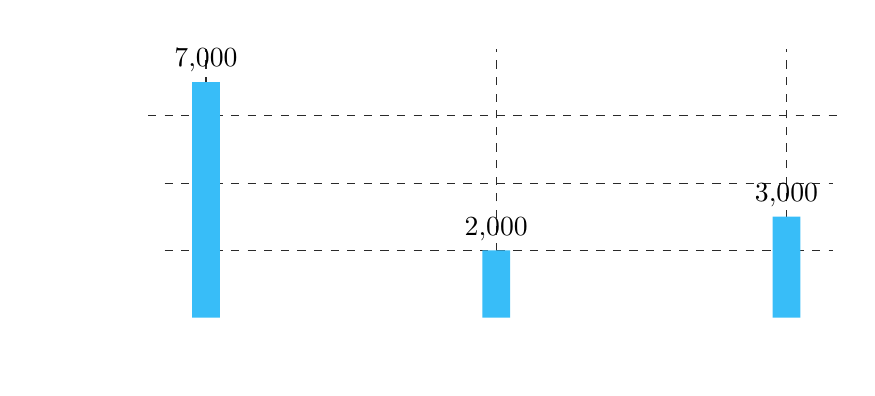
\begin{tikzpicture}
\begin{axis}[
  ybar,
  width=0.86\linewidth, height=5.0cm,
  ymin=0, ymax=8000,
  symbolic x coords={Jackets,Sweaters,Trousers},
  xtick=data,
  ylabel={Number of items},
  nodes near coords,
  grid=major,
  grid style={dashed, border},
]
\addplot[fill=cyan, draw=none] coordinates {(Jackets,7000) (Sweaters,2000) (Trousers,3000)};
\end{axis}
\end{tikzpicture}
\end{center}

\end{QAPair}

% ============================================================
% Q3
\begin{QAPair}{Question 3}
\textcolor{gold}{\bfseries Question:} A number wheel has $8$ equal sectors labelled: pansy, lily, orchid, tulip, jasmine, rose, marigold, sunflower. Find probability that the pointer:
(i) stops at rose \quad (ii) stops at a 4-letter flower name \quad (iii) does not stop at marigold\\
(iv) stops at a 3-letter flower name \quad (vi) stops at a flower name
\tcblower
\textcolor{green}{\bfseries Answer:}

\begin{SetupBox}{Setup (8 equal sectors)}
\Step{1} Total outcomes $|\Samp|=8$ (because there are 8 equal sectors).\\[4pt]
\textbf{(Diagram) Spinner wheel}
\begin{center}
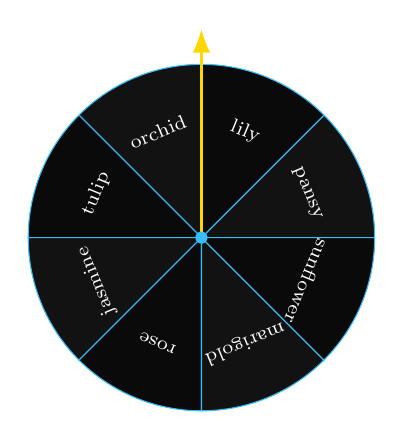
\begin{tikzpicture}[scale=1]
\def\R{2.2}
\foreach \i/\name in {
  0/pansy,45/lily,90/orchid,135/tulip,180/jasmine,225/rose,270/marigold,315/sunflower}{
  \pgfmathparse{mod(int(\i/45),2)==0 ? "pairbg" : "solbg"}
  \edef\fillcol{\pgfmathresult}
  \draw[draw=cyan, fill=\fillcol] (0,0) -- (\i:\R) arc (\i:\i+45:\R) -- cycle;
}
\foreach \i/\name in {
  22.5/pansy,67.5/lily,112.5/orchid,157.5/tulip,202.5/jasmine,247.5/rose,292.5/marigold,337.5/sunflower}{
  \node[text=text, font=\scriptsize, rotate=\i-90] at (\i:1.45) {\name};
}
\draw[-{Latex[length=3mm]}, line width=0.9pt, color=gold] (0,0) -- (90:2.65);
\fill[cyan] (0,0) circle (2.2pt);
\end{tikzpicture}
\end{center}
\end{SetupBox}

\begin{PartBox}{(i) Stops at \textbf{rose}}
\Step{1} Total outcomes $=8$.\\
\Step{2} Rose is only \textbf{one} sector $\Rightarrow$ favourable $=1$.\\
\Step{3} Divide:
\[
\Pof{\text{rose}}=\frac{1}{8}.
\]
\end{PartBox}

\begin{PartBox}{(ii) Stops at a \textbf{4-letter} flower name}
\Step{1} Count letters: lily (4), rose (4).\\
\Step{2} Favourable outcomes $=2$ sectors.\\
\Step{3} Divide and simplify:
\[
\Pof{\text{4-letter}}=\frac{2}{8}=\frac{1}{4}.
\]
\end{PartBox}

\begin{PartBox}{(iii) \textbf{Does not} stop at marigold}
\Step{1} Marigold is 1 sector, so $\Pof(\text{marigold})=\frac{1}{8}$.\\
\Step{2} Use complement:
\[
\Pof(\text{not marigold})=1-\frac{1}{8}=\frac{7}{8}.
\]
\end{PartBox}

\begin{PartBox}{(iv) Stops at a \textbf{3-letter} flower name}
\Step{1} Look at the names: none has 3 letters.\\
\Step{2} Favourable outcomes $=0$.\\
\Step{3} Divide:
\[
\Pof(\text{3-letter})=\frac{0}{8}=0.
\]
\end{PartBox}

\begin{PartBox}{(vi) Stops at a \textbf{flower name}}
\Step{1} All 8 sectors are flower names.\\
\Step{2} Favourable outcomes $=8$.\\
\Step{3} Divide:
\[
\Pof(\text{flower name})=\frac{8}{8}=1.
\]
\end{PartBox}

\end{QAPair}

% ============================================================
% Q4
\begin{QAPair}{Question 4}
\textcolor{gold}{\bfseries Question:} A decagonal die labelled $4,4,4,4,5,5,6,7,8,8$ is rolled once. Find probability of getting:
(i) a 4 \quad (ii) an even number \quad (iii) a multiple of 4 \quad (iv) not a 7 \quad (v) an odd number\\
(vi) a prime number \quad (vii) LCM of 4 and 8 \quad (viii) HCF of 4 and 8 \quad (ix) factor of 12
\tcblower
\textcolor{green}{\bfseries Answer:}

\begin{SetupBox}{Setup (count each face)}
Total outcomes $=10$.
\begin{center}
\DarkTable
\begin{tabular}{c c}
\rowcolor{tablehead}\textcolor{text}{\textbf{Number}} & \textcolor{text}{\textbf{Count}}\\
$4$ & $4$\\
$5$ & $2$\\
$6$ & $1$\\
$7$ & $1$\\
$8$ & $2$\\
\rowcolor{tablehead}\textcolor{text}{\textbf{Total}} & \textcolor{text}{\bfseries 10}\\
\end{tabular}
\end{center}
\textbf{Tip:} Probability $=$ (count) $\div 10$.
\end{SetupBox}

\begin{PartBox}{(i) Getting a 4}
\Step{1} Count of 4 is $4$.\\
\Step{2} Divide by 10:
\[
\Pof{4}=\frac{4}{10}=\frac{2}{5}.
\]
\end{PartBox}

\begin{PartBox}{(ii) Getting an even number}
Even numbers here are $4,6,8$.\\
\Step{1} Count $=4+1+2=7$.\\
\Step{2} Divide:
\[
\Pof(\text{even})=\frac{7}{10}.
\]
\end{PartBox}

\begin{PartBox}{(iii) Getting a multiple of 4}
Multiples of 4 here are $4$ and $8$.\\
\Step{1} Count $=4+2=6$.\\
\Step{2} Divide:
\[
\Pof(\text{multiple of }4)=\frac{6}{10}=\frac{3}{5}.
\]
\end{PartBox}

\begin{PartBox}{(iv) Getting \textbf{not} a 7}
\Step{1} Count of 7 is $1$, so “not 7” count is $10-1=9$.\\
\Step{2} Divide:
\[
\Pof(\text{not }7)=\frac{9}{10}.
\]
\end{PartBox}

\begin{PartBox}{(v) Getting an odd number}
Odd numbers here are $5$ and $7$.\\
\Step{1} Count $=2+1=3$.\\
\Step{2} Divide:
\[
\Pof(\text{odd})=\frac{3}{10}.
\]
\end{PartBox}

\begin{PartBox}{(vi) Getting a prime number}
Prime numbers here are $5$ and $7$ (4,6,8 are not prime).\\
\Step{1} Count $=2+1=3$.\\
\Step{2} Divide:
\[
\Pof(\text{prime})=\frac{3}{10}.
\]
\end{PartBox}

\begin{PartBox}{(vii) Getting LCM of 4 and 8}
\Step{1} LCM$(4,8)=8$.\\
\Step{2} Count of 8 is $2$.\\
\Step{3} Divide:
\[
\Pof(8)=\frac{2}{10}=\frac{1}{5}.
\]
\end{PartBox}

\begin{PartBox}{(viii) Getting HCF of 4 and 8}
\Step{1} HCF$(4,8)=4$.\\
\Step{2} Count of 4 is $4$.\\
\Step{3} Divide:
\[
\Pof(4)=\frac{4}{10}=\frac{2}{5}.
\]
\end{PartBox}

\begin{PartBox}{(ix) Getting a factor of 12}
Factors of 12 are $1,2,3,4,6,12$. From the die, only $4$ and $6$ are factors.\\
\Step{1} Count of $4$ and $6$ is $4+1=5$.\\
\Step{2} Divide:
\[
\Pof(\text{factor of }12)=\frac{5}{10}=\frac{1}{2}.
\]
\end{PartBox}

\textbf{(Diagram) Face counts}
\begin{center}
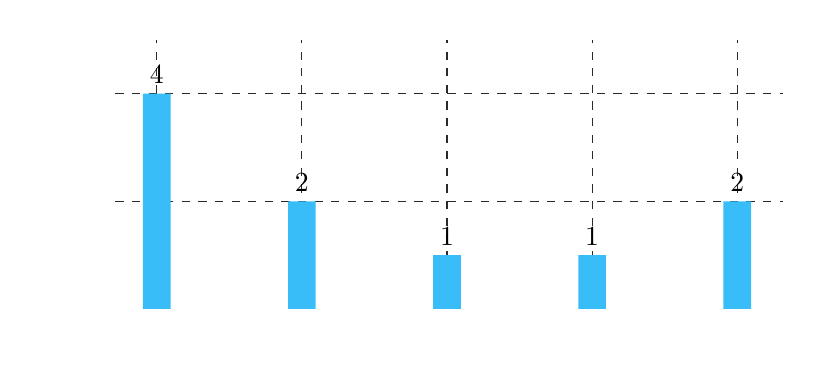
\begin{tikzpicture}
\begin{axis}[
  ybar,
  width=0.86\linewidth, height=5.0cm,
  ymin=0, ymax=5,
  symbolic x coords={4,5,6,7,8},
  xtick=data,
  ylabel={Count on die},
  nodes near coords,
  grid=major,
  grid style={dashed, border},
]
\addplot[fill=cyan, draw=none] coordinates {(4,4) (5,2) (6,1) (7,1) (8,2)};
\end{axis}
\end{tikzpicture}
\end{center}

\end{QAPair}

% ============================================================
% Q5
\begin{QAPair}{Question 5}
\textcolor{gold}{\bfseries Question:} A one-digit whole number is chosen at random. Find probability that it is:
(i) less than 5 \quad (ii) greater than 10 \quad (iii) not the largest 1-digit number\\
(iv) additive identity of whole numbers \quad (v) HCF of 3 and 5 \quad (vi) multiplicative identity of real numbers\\
(vii) not a prime number \quad (viii) factor of 9
\tcblower
\textcolor{green}{\bfseries Answer:}

\begin{SetupBox}{Setup (sample space 0 to 9)}
\[
\Samp=\{0,1,2,3,4,5,6,7,8,9\},\qquad |\Samp|=10
\]
\textbf{(Diagram) Number line (primes marked in cyan)}
\begin{center}
\begin{tikzpicture}
\draw[->, color=text, line width=0.7pt] (-0.5,0) -- (9.8,0);
\foreach \x in {0,1,2,3,4,5,6,7,8,9}{
  \draw[color=text] (\x,0.08) -- (\x,-0.08);
  \node[below, text=text, font=\small] at (\x,-0.08) {\x};
}
\foreach \x in {2,3,5,7}{\fill[cyan] (\x,0) circle (2.0pt);}
\node[above, text=muted, font=\small] at (4.5,0.35) {Primes: 2, 3, 5, 7};
\end{tikzpicture}
\end{center}
\end{SetupBox}

\begin{PartBox}{(i) Less than 5}
Numbers are $\{0,1,2,3,4\}$ so favourable $=5$.\\
\[
\Pof(<5)=\frac{5}{10}=\frac{1}{2}.
\]
\end{PartBox}

\begin{PartBox}{(ii) Greater than 10}
No one-digit whole number is greater than 10, so favourable $=0$.\\
\[
\Pof(>10)=0.
\]
\end{PartBox}

\begin{PartBox}{(iii) Not the largest 1-digit number}
Largest one-digit number is $9$. “Not 9” means the other 9 numbers.\\
\[
\Pof(\text{not }9)=\frac{9}{10}.
\]
\end{PartBox}

\begin{PartBox}{(iv) Additive identity of whole numbers}
Additive identity is $0$.\\
\[
\Pof(0)=\frac{1}{10}.
\]
\end{PartBox}

\begin{PartBox}{(v) HCF of 3 and 5}
HCF$(3,5)=1$.\\
\[
\Pof(1)=\frac{1}{10}.
\]
\end{PartBox}

\begin{PartBox}{(vi) Multiplicative identity of real numbers}
Multiplicative identity is $1$.\\
\[
\Pof(1)=\frac{1}{10}.
\]
\end{PartBox}

\begin{PartBox}{(vii) Not a prime number}
Primes are $\{2,3,5,7\}$ (4 numbers).\\
So not-prime count $=10-4=6$.\\
\[
\Pof(\text{not prime})=\frac{6}{10}=\frac{3}{5}.
\]
\end{PartBox}

\begin{PartBox}{(viii) Factor of 9}
Factors of 9 (in 0--9) are $\{1,3,9\}$ so favourable $=3$.\\
\[
\Pof(\text{factor of }9)=\frac{3}{10}.
\]
\end{PartBox}

\end{QAPair}

% ============================================================
% Q6
\begin{QAPair}{Question 6}
\textcolor{gold}{\bfseries Question:} A coin is tossed $10$ times. Head $=6$, Tail $=4$. Complete the table and find expected frequencies for:
(i) $520$ tosses (Head) \quad (ii) $305$ tosses (Tail)
\tcblower
\textcolor{green}{\bfseries Answer:}

\begin{SetupBox}{Setup (relative/experimental probability)}
\Step{1} Total tosses $=10$.\\
\Step{2} Relative frequency:
\[
\Pof(H)=\frac{6}{10}=0.6,\qquad \Pof(T)=\frac{4}{10}=0.4.
\]
\Step{3} Complete table:
\begin{center}
\DarkTable
\begin{tabular}{l c c}
\rowcolor{tablehead}\textcolor{text}{\textbf{Event}} & \textcolor{text}{\textbf{Frequency}} & \textcolor{text}{\textbf{Relative frequency}}\\
Head & $6$ & $\dfrac{6}{10}=0.6$\\
Tail & $4$ & $\dfrac{4}{10}=0.4$\\
\end{tabular}
\end{center}
\end{SetupBox}

\begin{PartBox}{(i) Expected heads in 520 tosses}
\Step{1} Use Expected $= N \times \Pof(H)$.\\
\Step{2} $N=520$, $\Pof(H)=0.6$.\\
\[
\text{Expected heads}=520\times 0.6=\mathbf{312}.
\]
\end{PartBox}

\begin{PartBox}{(ii) Expected tails in 305 tosses}
\Step{1} Use Expected $= N \times \Pof(T)$.\\
\Step{2} $N=305$, $\Pof(T)=0.4$.\\
\[
\text{Expected tails}=305\times 0.4=\mathbf{122}.
\]
\end{PartBox}

\end{QAPair}

% ============================================================
% Q7
\begin{QAPair}{Question 7}
\textcolor{gold}{\bfseries Question:} A die is rolled $120$ times and frequencies are:
1:15,\; 2:25,\; 3:15,\; 4:20,\; 5:30,\; 6:15.\\
Complete the table and answer:
(i) if rolled $6000$ times, expected 6s
(ii) if rolled $3000$ times, expected 1s
(iii) if rolled $400$ times, expected 2s
\tcblower
\textcolor{green}{\bfseries Answer:}

\begin{SetupBox}{Setup (relative frequencies)}
\Step{1} Relative frequency $= \dfrac{f}{120}$.\\[2pt]
\begin{center}
\DarkTable
\begin{tabular}{c c c}
\rowcolor{tablehead}\textcolor{text}{\textbf{Number}} & \textcolor{text}{\textbf{Frequency}} & \textcolor{text}{\textbf{Relative frequency}}\\
$1$ & $15$ & $\dfrac{15}{120}=\dfrac18=0.125$\\
$2$ & $25$ & $\dfrac{25}{120}=\dfrac{5}{24}\approx 0.2083$\\
$3$ & $15$ & $\dfrac{15}{120}=\dfrac18=0.125$\\
$4$ & $20$ & $\dfrac{20}{120}=\dfrac16\approx 0.1667$\\
$5$ & $30$ & $\dfrac{30}{120}=\dfrac14=0.25$\\
$6$ & $15$ & $\dfrac{15}{120}=\dfrac18=0.125$\\
\rowcolor{tablehead}\textcolor{text}{\textbf{Total}} & \textcolor{text}{\bfseries 120} & \textcolor{text}{\bfseries 1}\\
\end{tabular}
\end{center}
\end{SetupBox}

\begin{PartBox}{(i) Expected number of 6s in 6000 rolls}
\Step{1} $\Pof(6)=\dfrac{15}{120}=\dfrac18$.\\
\Step{2} Expected $=6000\times \dfrac18$.
\[
\text{Expected 6s}=\mathbf{750}.
\]
\end{PartBox}

\begin{PartBox}{(ii) Expected number of 1s in 3000 rolls}
\Step{1} $\Pof(1)=\dfrac{15}{120}=\dfrac18$.\\
\Step{2} Expected $=3000\times \dfrac18$.
\[
\text{Expected 1s}=\mathbf{375}.
\]
\end{PartBox}

\begin{PartBox}{(iii) Expected number of 2s in 400 rolls}
\Step{1} $\Pof(2)=\dfrac{25}{120}=\dfrac{5}{24}$.\\
\Step{2} Expected $=400\times \dfrac{5}{24}$.
\[
\text{Expected 2s}= \frac{2000}{24}=\frac{250}{3}\approx \mathbf{83.33}\ (\text{about }83).
\]
\end{PartBox}

\textbf{(Diagram) Relative frequency bar chart}
\begin{center}
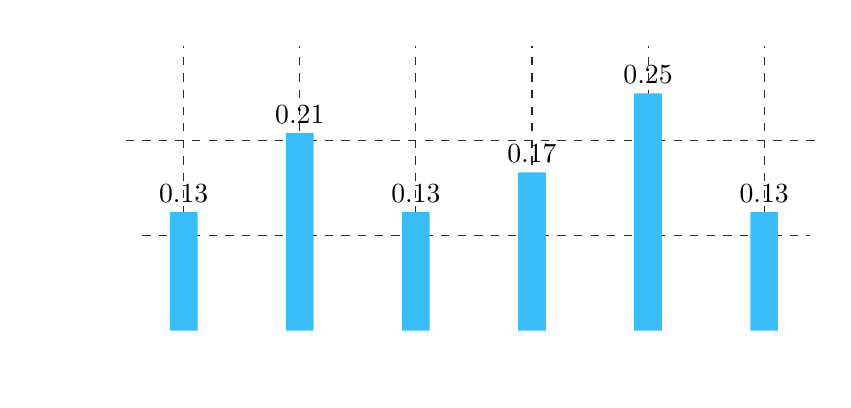
\begin{tikzpicture}
\begin{axis}[
  ybar,
  width=0.86\linewidth, height=5.2cm,
  ymin=0, ymax=0.30,
  symbolic x coords={1,2,3,4,5,6},
  xtick=data,
  ylabel={Relative frequency},
  nodes near coords,
  nodes near coords align={vertical},
  grid=major,
  grid style={dashed, border},
]
\addplot[fill=cyan, draw=none] coordinates
{(1,0.125) (2,0.208333) (3,0.125) (4,0.166667) (5,0.25) (6,0.125)};
\end{axis}
\end{tikzpicture}
\end{center}

\end{QAPair}

% ============================================================
% Q8
\begin{QAPair}{Question 8}
\textcolor{gold}{\bfseries Question:} There are $6$ girls sections: Teal, Orchid, Mauve, Hazel, Zaffre, Denim. One girl is chosen randomly from all sections.
(a) $\Pof(\text{Hazel})$ \quad (b) $\Pof(\text{Not Hazel})$ \quad (c) Verify unity \quad
(d) Expected Orchid (6 selections) \quad (e) Expected Teal (60 selections)
\tcblower
\textcolor{green}{\bfseries Answer:}

\begin{SetupBox}{Setup (equal chance for each section)}
There are $6$ sections and each section has equal chance, so:
\[
\Pof(\text{any one section})=\frac{1}{6}.
\]
\textbf{(Diagram) 6 equal section blocks (Hazel highlighted)}
\begin{center}
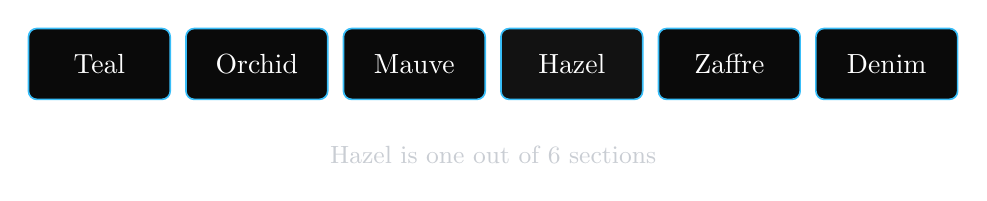
\begin{tikzpicture}
\foreach \i/\name in {0/Teal,1/Orchid,2/Mauve,3/Hazel,4/Zaffre,5/Denim}{
  \node[tile, minimum width=18mm, minimum height=9mm,
        fill={\ifnum\i=3 pairbg\else solbg\fi}] at (\i*2.0,0) {\name};
}
\node[below=9pt, text=muted, font=\small] at (5.0,-0.6) {Hazel is one out of 6 sections};
\end{tikzpicture}
\end{center}
\end{SetupBox}

\begin{PartBox}{(a) Probability of selecting Hazel}
\Step{1} Hazel is 1 section out of 6.\\
\[
\Pof(\text{Hazel})=\mathbf{\frac{1}{6}}.
\]
\end{PartBox}

\begin{PartBox}{(b) Probability of \emph{not} selecting Hazel}
\Step{1} Use complement:
\[
\Pof(\text{Not Hazel})=1-\frac{1}{6}=\mathbf{\frac{5}{6}}.
\]
\end{PartBox}

\begin{PartBox}{(c) Verify that answers add up to unity (1)}
\Step{1} Add:
\[
\frac{1}{6}+\frac{5}{6}=\frac{6}{6}=\mathbf{1}.
\]
So, verified.
\end{PartBox}

\begin{PartBox}{(d) Expected Orchid selections if 6 girls are selected}
\Step{1} $\Pof(\text{Orchid})=\frac{1}{6}$.\\
\Step{2} Expected $=6\times \frac{1}{6}$.
\[
\text{Expected Orchid}=\mathbf{1}.
\]
\end{PartBox}

\begin{PartBox}{(e) Expected Teal selections if 60 girls are selected}
\Step{1} $\Pof(\text{Teal})=\frac{1}{6}$.\\
\Step{2} Expected $=60\times \frac{1}{6}$.
\[
\text{Expected Teal}=\mathbf{10}.
\]
\end{PartBox}

\end{QAPair}

\end{document}
